\documentclass[border=5mm]{standalone}
  \usepackage{tikz}
  \usetikzlibrary{optics}
  \usepackage{tikzpeople}
  
\begin{document}
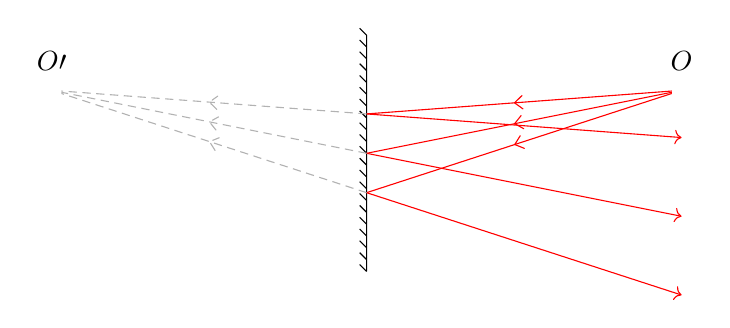
\begin{tikzpicture}[use optics]
	\node[mirror, object height=3cm, rotate=180] at (5,0) {};

	\node (O) at (9,0.8) [label=$O$]{};
	\node (O') at (1,0.8) [label={$O\prime$}]{};

	% red ray
	\begin{scope}[red]
		% rays
		\draw[->-] (O) -- (5,0.5) coordinate (C1);
		\draw[->-] (O) -- (5,-0) coordinate (C2);
		\draw[->-] (O) -- (5,-0.5) coordinate (C3);

		\draw[->] (C1) -- (9, 0.2);
		\draw[->] (C2) -- (9, -0.8);
		\draw[->] (C3) -- (9, -1.8);
	\end{scope}

	% image
	\draw[->-, densely dashed,gray!60] (C1) -- (O');
	\draw[->-, densely dashed,gray!60] (C2) -- (O');
	\draw[->-, densely dashed,gray!60] (C3) -- (O');

\end{tikzpicture}
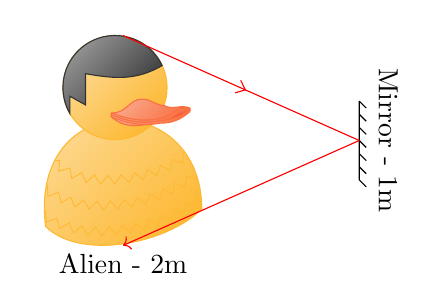
\begin{tikzpicture}[use optics]
  
  \node[mirror, object height=1cm] at (5,0) {};
  \node[label=right:\rotatebox{-90}{Mirror - 1m}] at (5,0) {};
  
  \node[duck,name=a,minimum size=2cm] at (2,0) {Alien - 2m};
  
  \begin{scope}[red]
    \draw[->-] (a.north) -- (5,0);
    \draw[->] (5,0) -- (a.south);
  \end{scope}
  
  \end{tikzpicture}
\end{document}